
\begin{frame}
	\frametitle{Reconnaître la Langue grâce à des caractéristiques statistiques}

\textcolor{blue}{Loi de Zipf} :
\begin{itemize}
\item ``the'' représente près de 7~\% du \textit{Brown Corpus\footnote{1 million de mots} };
\item 135 mots représentent la moitié des occurrences du \textit{Brown Corpus};
\item Inversement, la moitié du vocabulaire du corpus sont des \textcolor{red}{hapax}; 
%\item \textbf{proportionnalité} entre rang et effectif; 
\item \textbf{proportionnalité} entre rang ($r$) et fréquence ($f$)
\item Les mots fréquents sont très rares\dots et inversement.
\end{itemize}   

\begin{center}
\begin{table}[ht]
 \begin{tabular}{|c|c|c|l|}
\hline
Rang ($r$) & Mot & Fréquence  ($f$)		& ratio 	\\
\hline
1 & \textit{the}  & 69~971 	& \\
\hline
2 & \textit{of} & 36~412 	& 1,94 fois moins\\
\hline
3 & \textit{and} &  28~853 	& 2,41 fois moins\\
\hline
... & ... & ... 	&...\\
\hline
20  & \textit{I}  & 5~164 	& 13,72 fois moins \dots\\
\hline
\end{tabular} 
\end{table}
\end{center}

\end{frame}


 \begin{frame}
   \frametitle{Loi de Zipf sur le \textit{Brown corpus}}
\begin{figure}
\begin{center}
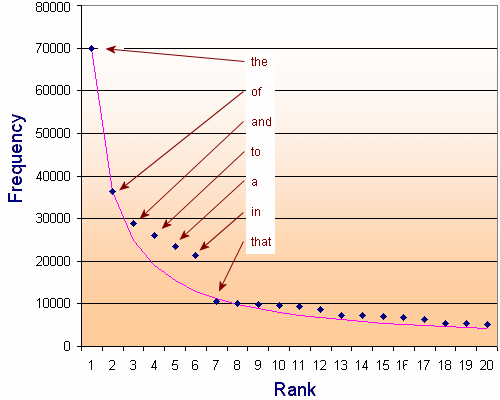
\includegraphics[width=6cm]{images/zipf.png}
\end{center}   
\caption{Données très proches de l'attendu, surtout sur la longue traîne}
\end{figure}
\end{frame}

 \begin{frame}
   \frametitle{Loi de Zipf sur le \textit{Brown corpus}}
\begin{figure}
 \begin{center}
  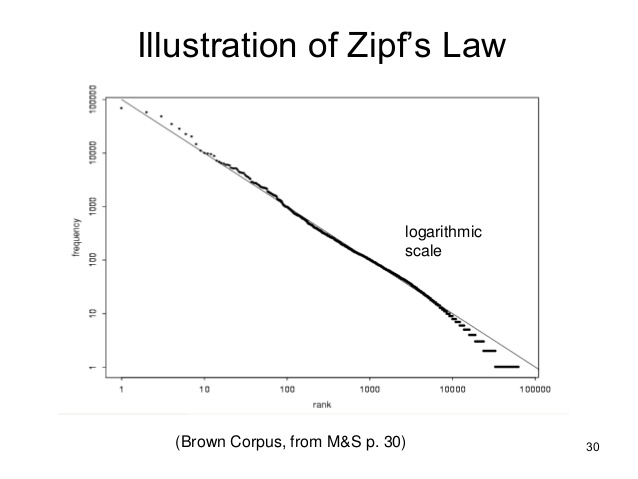
\includegraphics[width=6cm]{images/zipf2.jpg}
 \end{center}   
\caption{Validité plus marquante encore en échelle logarithmique}
\end{figure}
\end{frame}

\begin{frame}
   \frametitle{Identifier la langue : solution simple}
 Méthode des  \textit{short words} / \textit{frequent words} :
\begin{itemize}
\item Liste de "mots outils" (mots grammaticaux, "petits" mots) pour chaque langue
\item Compter les occurrences de ces mots outils dans le texte     
\item Comparer avec des listes de référence
\end{itemize}
   
\end{frame}

\begin{frame}

\frametitle{Implantation rapide (POC)}

\begin{block}{Données: corpus parallèle de l'Union Européenne (22 langues)}

\begin{itemize}
  \item Découpage en deux parties (entraînement et test)
  \item Entraînement : extraction d'un modèle de langue ( les $n$ mots les plus fréquents) à partir de tous les textes de chaque langue
\pause
  \item Test, pour chaque texte :
  \begin{itemize}
    \item calcul de l'intersection en mots
    \item on prend la plus grande $\rightarrow$ prédiction
  \end{itemize}
\end{itemize}

\end{block}
\end{frame}

\begin{frame}
\frametitle{Les modèles}
\begin{small}
\input{ressources/tabs/langid_ref}
\end{small}
\end{frame}

\begin{frame}
\frametitle{L'application : des erreurs explicables}
\begin{small}
\input{ressources/tabs/langid_err}
\end{small}

\end{frame}

\begin{frame}
\frametitle{Autres Modèles : 3-grammes de caractère}
\begin{small}
\input{ressources/tabs/langid3GRAM_ref}
\end{small}
\end{frame}

\begin{frame}
  \frametitle{Bilan : ça marche !}

Plus de 96\% de bonne prédiction sur 22 langues, \texttt{langid.py} fait encore mieux. Plus rapide et plus efficace que l'humain.
\begin{block}{Mais pourquoi ?}

\pause

\begin{itemize}
  \item Des données disponibles
  \item Une tâche facile à définir (classification)
  \item Et facile à évaluer
  \pause
  \item Une théorie linguistique bien stable \dots
  \item \dots et facile à rendre calculable
\end{itemize}
\end{block}

%\bigskip
%\only<2>{
%$\rightarrow$ \textit{trishort}
%}
\end{frame}

